%{{{ Preamble

%\documentclass[draft]{beamer} %% normal document
\documentclass[]{beamer} %% normal document
\usepackage{fontspec, unicode-math, caption, float, filecontents, verbatim}
\usepackage[english]{babel}

%{{{ Beamer Stuff

\usetheme{Frankfurt}
\useoutertheme{split}
\useinnertheme{rectangles}
%%\definecolor{bettergreen}{rgb}{.1,.7,.1}
%%\usecolortheme[named=bettergreen]{beaver}

\definecolor{bettergreen}{rgb}{0.1,0.7,0.1}

%\usetheme{Dresden}
%\usecolortheme[named=bettergreen]{structure}
\usecolortheme[named=bettergreen]{structure}

\setbeamercolor{section in head/foot}{fg=green, bg=black}
\setbeamercolor{section shaded}{fg= grey}


%\setbeamertemplate{caption}[numbered]
%\captionsetup{labelformat=simple,font=scriptsize,labelfont=scriptsize}
\beamertemplatenavigationsymbolsempty

% puts Frame numbers in Dresden template
\newcommand*\oldmacro{}%
\let\oldmacro\insertshorttitle%
\renewcommand*\insertshorttitle{%
	\oldmacro\hfill%
\insertframenumber\,/\,\inserttotalframenumber}

%\logo{\pgfimage[width=2cm,height=2cm]{material/schlangenlogo}}
\newcommand{\nologo}{\setbeamertemplate{logo}{}} % command to set the logo to nothing


\AtBeginSection[]
{%
	\begin{frame}<beamer>
		\frametitle{Table of Contents}
		\tableofcontents[currentsection]
		%\tableofcontents
	\end{frame}
}




%}}}


\newcommand{\as}[1]{{\fontspec{ProFontWindows} \textcolor{white}{#1} } }
\newcommand{\source}[1]{{\caption{\tiny {\fontspec{ProFontWindows} {Source: #1} } } } }
\newcommand{\greenbullet}{\textcolor{bettergreen}\textbullet}
%\newcommand{\greencirc}{\textcolor{bettergreen} $ \circ $}
\newcommand{\greencirc}{$ \circ $ }

\usepackage{multicol}



%{{{ Avebritations

\usepackage{xspace}
\newcommand{\twi}{I\textsuperscript{2}C\xspace}
\newcommand{\mosi}{\texttt{MOSI}\xspace}
\newcommand{\miso}{\texttt{MISO}\xspace}
\newcommand{\clock}{\texttt{CLOCK}\xspace}
\renewcommand{\ss}{\texttt{\textoverline{SS}}\xspace}

\newcommand{\sda}{\texttt{SDA}\xspace}
\newcommand{\scl}{\texttt{SCL}\xspace}
\newcommand{\startcondition}{\texttt{START} condition\xspace}
\newcommand{\stopcondition}{\texttt{STOP} condition\xspace}
\newcommand{\clockstretching}{\texttt{CLOCK STRETCHING}\xspace}
\newcommand{\ack}{\texttt{ACK}\xspace}
\newcommand{\nak}{\texttt{NACK}\xspace}
%}}}

%{{{ Title

\title[]{Industry Standard Control Interfaces for inter IC Communication}
%\subtitle[]{Presenting SPI and \twi}
%\subject{}
\keywords{System buses, SPI, \twi, Two Wire Interface}
\date{\today}
%}}}

%{{{ Author

\author{Moritz~Nöltner}
\institute[ZITI]}}

%{{{ MINTED

\usepackage{minted}
\definecolor{bg}{rgb}{0.95,0.95,0.95}
%\newminted[C++]{cpp}{numbersep=5pt, bgcolor=bg, gobble=0, linenos, tabsize=4}
%\newminted[C++]{cpp}{tabsize=4, obeytabs}
%}}} Minted

%{{{ Hyperref

\usepackage{hyperref}
\definecolor{darkblue}{rgb}{0,0,.5}
%linkcolor will also affect the text in the navigation bar on the top of each slide
%\hypersetup{pdftex=true, colorlinks=true, breaklinks=true, linkcolor=darkblue, menucolor=darkblue, pagecolor=darkblue, urlcolor=darkblue}
%}}}

%{{{ Animate

%%\usepackage[controls, autoplay]{animate}
%\usepackage[autoplay]{animate}
%%\animategraphics[<options>]{<frameand the environment rate>}{<file basename>}{<first>}{<last>}
%}}}

%{{{ Changemargin

\newenvironment{changemargin}[2]
{
	\begin{list}{}
		{
			\setlength{\topsep}{0pt}
			\setlength{\leftmargin}{#1}
			\setlength{\rightmargin}{#2}
			\setlength{\listparindent}{\parindent}
		\setlength{\itemindent}{\parindent}
			\setlength{\parsep}{\parskip}
		}
	\item[]
	}
	{
	\end{list}
}
%}}}

%{{{ Graphics Loading

\usepackage{graphicx}
\graphicspath{{../material/presentation/}}
\usepackage{caption}
\captionsetup[figure]{labelformat=empty, font=scriptsize, justification=raggedleft, singlelinecheck=false}% redefines the caption setup of the figures environment in the beamer class.
%}}}

%{{{ Tkz drawing package

%{{{ Spider diagram

%\usepackage{tkz-kiviat,numprint,fullpage}
\usepackage{tkz-kiviat,numprint}
\usetikzlibrary{arrows}
%}}}

%{{{ Block diagram

\usepackage{tikz}
\usetikzlibrary{arrows, decorations.markings, positioning}

% for double arrows a la chef
% adapt line thickness and line width, if needed
\tikzstyle{vecArrow} = [thick, decoration={markings,mark=at position
	1 with {\arrow[semithick]{open triangle 60} } },
	double distance=1.4pt, shorten >= 5.5pt,
	preaction = {decorate},
postaction = {draw,line width=1.4pt, white,shorten >= 4.5pt}]
\tikzstyle{innerWhite} = [semithick, white,line width=1.4pt, shorten >= 4.5pt]
%}}}

%{{{ Tkz timing package

\usepackage{tikz-timing}
%\usetikztiminglibrary{nicetabs} % a bit strange with \Huge; use belowrulesep to adjust
%}}}

%}}}

%}}}




%{{{
\begin{document}

%{{{ Titlepage

\begin{frame}[plain]
	\titlepage
	%\note{}
\end{frame}
%}}}

%{{{ Table of Contents

\begin{frame}<beamer>
	\frametitle{Table of Contents}
	\tableofcontents
\end{frame}
%}}}




\section{Introduction}

%{{{
\begin{frame}{How to Connect Circuits?}
	\begin{figure}
		\centering
		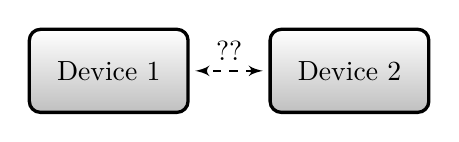
\begin{tikzpicture}[node distance=1cm, auto]
			\tikzset{%
				mynode/.style={rectangle,rounded corners,draw=black,top color=white, bottom color=gray!50,very thick, inner sep=1em, minimum size=3em, text centered}
			}
			\node[mynode](dev1){Device 2};
			\node[mynode, left=of dev1](dev2){Device 1};
			\draw[<->, >=latex', shorten >=2pt, shorten <=2pt, thick, dashed] (dev1.west) to node[auto, swap] {??}(dev2.east); 
		\end{tikzpicture}
	\end{figure}
	\begin{columns}
		\column{0.6\textwidth}
		\begin{itemize}
			\item HyperTransport
			\item PATA, SATA
			\item PCI, PCI-Express
			\item AGP
			\item ISA
			\item USB
		\end{itemize}
		\column{0.4\textwidth}
		\begin{itemize}
			\item CAN
			\item UART, USART
			\item SPI
			\item \twi, SMBus
			\item UNI/O
			\item 1-Wire
		\end{itemize}
	\end{columns}
\end{frame}
%}}}

%{{{
\begin{frame}{Speed <=> Simplicity}
	\begin{figure}
		
\includegraphics[width=0.8\linewidth]{dummy}
		\source{\url{http://www.anandtech.com/show/2354/2}}
	\end{figure}
	%\note{v1 = Zielvektor\\k2 = Maskenregister\\rax = Basepointer\\v3 = Adressvektor}
\end{frame}
%}}}




\section[SPI]{Serial Peripheral Interface}

%{{{
\begin{frame}{Serial Peripheral Interface}
	\begin{columns}
		\column{0.6\textwidth}
		\begin{figure}
			
\includegraphics[width=0.9\linewidth]{dummy}
			\source{\url{http://en.wikipedia.org/wiki/File:Motorola_MC6800_microprocessor.jpg}}
		\end{figure}
		\column{0.4\textwidth}
		\begin{itemize}
			\item Created in the 1980s
			\item First used in Motorola 6800
			\item Very widely accepted
			\item Bus system
			\item Full duplex
			\item Four signal lines typically
		\end{itemize}
	\end{columns}
\end{frame}
%}}}

%{{{
\begin{frame}{SPI Signal Lines}
	\begin{figure}
		\centering
		\only<1>{
\includegraphics[width=0.9\linewidth]{dummy}}%
		\only<2>{
\includegraphics[width=0.9\linewidth]{dummy}}%
		\only<3>{
\includegraphics[width=0.9\linewidth]{dummy}}%
		\only<4>{
\includegraphics[width=0.9\linewidth]{dummy}}%
		\only<5>{
\includegraphics[width=0.9\linewidth]{dummy}}%
		\source{Adapted from \href{http://www.ee.nmt.edu/~teare/ee308l/datasheets/S12SPIV3.pdf}{``SPI Block Guide V 03.06'', 2003}}
	\end{figure}
	\vspace{1cm}
	\begin{tabular}{p{0.15cm} p{2.8cm} p{7cm}}
		\only<1>{\\}
		\only<1>{\\}

		\only<2>{\greenbullet & \ss & Slave Select\\}
		\only<2>{& & Slaves will only interact if their \ss is acrive\\}

		\only<3>{\greenbullet & \mosi & Master Out, Slave In\\}
		\only<3>{& & Serial data line for master to slave\\}

		\only<4>{\greenbullet & \miso & Master In, Slave Out\\}
		\only<4>{& & Serial data line for master to slave\\}

		\only<5>{\greenbullet & \clock & Shift Clock\\}
		\only<5>{& & One bit is sent per clock cycle\\}
		\\
	\end{tabular}
\end{frame}
%}}}

%{{{
\begin{frame}{Clock Phase \& Polarity}
	\centering
	{\Large 4 combinations:}
	\begin{figure}
		
\includegraphics[width=0.8\linewidth]{dummy}
		\source{Taken from \href{http://pdf.datasheetcatalog.com/datasheet/motorola/MC68HCP11A1VP.pdf}{the datasheet for Motorola MC68HC11A0}}
	\end{figure}
\end{frame}
%}}}

%{{{
\begin{frame}{SPI Bus Topologies: Star}
	\begin{columns}
		\column{0.5\textwidth}
		\begin{figure}
			
\includegraphics[width=0.9\linewidth]{dummy}
		\source{Adapted from \url{http://en.wikipedia.org/wiki/File:SPI_three_slaves.svg}}
		\end{figure}
		\column{0.5\textwidth}
		\begin{itemize}
			\item 3+n signal lines
			\item \mosi, \miso, \clock shared
			\item One \ss for every slave
			\item Master activates a slave and communicates with it
			\item No delay
		\end{itemize}
	\end{columns}
\end{frame}
%}}}

%{{{
\begin{frame}{SPI Bus Topologies: Serial}
	\begin{columns}<+->
		\column{0.5\textwidth}
		\begin{figure}
			
\includegraphics[width=0.9\linewidth]{dummy}
			\source{Adapted from \url{http://en.wikipedia.org/wiki/File:SPI_three_slaves_daisy_chained.svg}}
		\end{figure}
		\column{0.5\textwidth}
		\begin{itemize}
			\item Four signal lines
			\item \mosi, \miso, \clock, \ss shared
			\item Messages are passed through
			\item Messages get latched, when \ss is deasserted
			\item Not supported by all devices
			\item Delayed responses, message has to pass adjacent slaves
		\end{itemize}
	\end{columns}
\end{frame}
%}}}





\section[\twi]{Inter-Integrated Circuit}

%{{{
\begin{frame}{Inter-Integrated Circuit}
	\begin{columns}
		\column{0.6\textwidth}
		\begin{figure}
			
\includegraphics[width=0.9\linewidth]{dummy}
			\source{\url{http://www.cpushack.com/gallery-1/philips/philipsmab8400b}}
		\end{figure}
		\column{0.4\textwidth}
		\begin{itemize}
			\item Created in the 1980s
			\item First used in Philips MAB8400B
			\item Very widely accepted
			\item Compatible with other buses: SMBus, PMBus
			\item Bus system
			\item Multi-master operation
			\item Half duplex (simplex)
			\item Two signal lines + two pull-up resistors
		\end{itemize}
	\end{columns}
\end{frame}
%}}}

%{{{
\begin{frame}{\twi Roles}
	Four roles possible:
	\begin{tabular}{p{2.8cm} p{7cm}}
		\greenbullet Master & Starts a transmission\\
		\greenbullet Slave & Responds to transmission\\
		\greenbullet Transmitter & Transmits data\\
		\greenbullet Receiver & Receives data\\
	\end{tabular}
\end{frame}
%}}}

%{{{
\begin{frame}{\twi Signal Lines}
	\begin{figure}
		\centering
		\only<1>{
\includegraphics[width=0.9\linewidth]{dummy}}%
		\only<2>{
\includegraphics[width=0.9\linewidth]{dummy}}%
		\only<3>{
\includegraphics[width=0.9\linewidth]{dummy}}%
		\source{Adapted from \href{http://www.cs.unc.edu/Research/stc/FAQs/Interfaces/I2C-BusSpec-V2.1.pdf}{``The I\textsuperscript{2}C-Bus Specification v. 2.1'', 2000}}
	\end{figure}
	\vspace{1cm}
	\begin{tabular}{p{2.8cm} p{7cm}}
		\only<1>{\\}
		\only<1>{\\}
		\only<1>{\\}
		\only<2>{\greenbullet \sda & Seria Data\\}
		\only<2>{& Bidirectional data-- \& address line\\}
		\only<2>{\\}
		\only<3>{\greenbullet \scl & Serial Clock\\}
		\only<3>{& Used by the master to synchronise with the slaves\\}
		\\
	\end{tabular}
\end{frame}
%}}}

%{{{
\begin{frame}{\twi Electrical Setup}
	\begin{columns}
		\column{0.6\textwidth}
		\begin{figure}
			
\includegraphics[width=\textwidth,height=0.7\textheight,keepaspectratio]{dummy}
			\source{Adapted from \href{http://www.cs.unc.edu/Research/stc/FAQs/Interfaces/I2C-BusSpec-V2.1.pdf}{``The I\textsuperscript{2}C-Bus Specification v. 2.1'', 2000}}
		\end{figure}
		\column{0.4\textwidth}
		\begin{itemize}
			\item Open-drain or open-collector outputs
			\item Wired-AND
		\end{itemize}
	\end{columns}
\end{frame}
%}}}

%{{{
\begin{frame}{\twi Protocol Parts}
	\begin{minipage}[c][.35\textheight][c]{\linewidth}
	%{{{
		\only<1>{%
			\begin{figure}
				\centering
				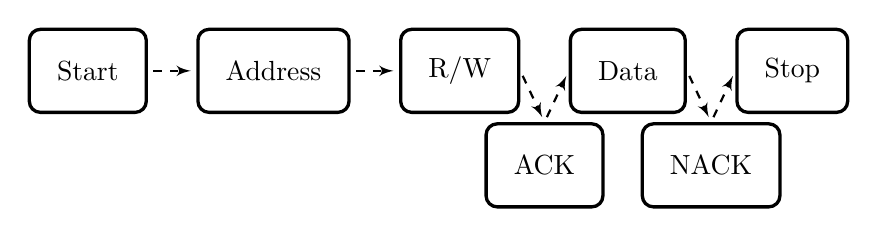
\begin{tikzpicture}[node distance=0.3cm, auto]
					\tikzset{%
						mynode/.style={rectangle,rounded corners,draw=black,top color=white, bottom color=white!50,very thick, inner sep=1em, minimum size=3em, text centered},
						invnode/.style={inner sep=0,minimum size=0}
					}
					\node[mynode](s){Start};
					\node[invnode, right=of s](i1){};
					\node[mynode, right=of i1](a){Address};
					\node[invnode, right=of a](i2){};
					\node[mynode, right=of i2](r){R/\textoverline{W}};
					\node[invnode, right=of r](i3){};
					\node[invnode, below of=i3](iv1){};
					\node[invnode, below of=iv1](iv2){};
					\node[invnode, below of=iv2](iv3){};
					\node[mynode, below of=iv3](ack1){ACK};
					\node[mynode, right=of i3](d){Data};
					\node[invnode, right=of d](i4){};
					\node[invnode, below of=i4](iv4){};
					\node[invnode, below of=iv4](iv5){};
					\node[invnode, below of=iv5](iv6){};
					\node[mynode, below of=iv6](ack2){NACK};
					\node[mynode, right=of i4](p){Stop};

					\draw[->, >=latex', shorten >=2pt, shorten <=2pt, thick, dashed] (s.east) to node[auto, swap] {}(a.west); 
					\draw[->, >=latex', shorten >=2pt, shorten <=2pt, thick, dashed] (a.east) to node[auto, swap] {}(r.west); 
					\draw[->, >=latex', shorten >=2pt, shorten <=2pt, thick, dashed] (r.east) to node[auto, swap] {}(ack1.north); 
					\draw[->, >=latex', shorten >=2pt, shorten <=2pt, thick, dashed] (ack1.north) to node[auto, swap] {}(d.west); 
					\draw[->, >=latex', shorten >=2pt, shorten <=2pt, thick, dashed] (d.east) to node[auto, swap] {}(ack2.north); 
					\draw[->, >=latex', shorten >=2pt, shorten <=2pt, thick, dashed] (ack2.north) to node[auto, swap] {}(p.west); 
				\end{tikzpicture}
			\end{figure}
		}
	%}}}
	%{{{
		\only<2>{%
			\begin{figure}
				\centering
				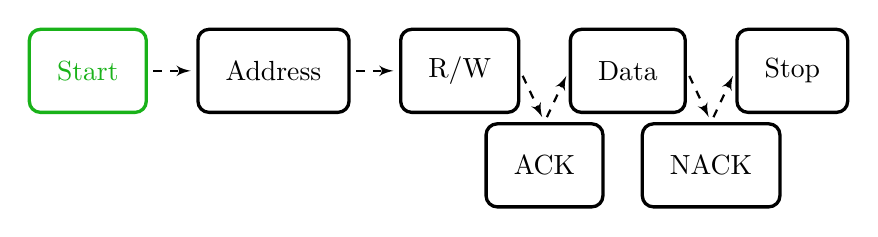
\begin{tikzpicture}[node distance=0.3cm, auto]
					\tikzset{%
						mynode/.style={rectangle,rounded corners,draw=black,top color=white, bottom color=white!50,very thick, inner sep=1em, minimum size=3em, text centered},
						invnode/.style={inner sep=0,minimum size=0}
					}
					\node[mynode,color=bettergreen](s){Start};
					\node[invnode, right=of s](i1){};
					\node[mynode, right=of i1](a){Address};
					\node[invnode, right=of a](i2){};
					\node[mynode, right=of i2](r){R/\textoverline{W}};
					\node[invnode, right=of r](i3){};
					\node[invnode, below of=i3](iv1){};
					\node[invnode, below of=iv1](iv2){};
					\node[invnode, below of=iv2](iv3){};
					\node[mynode, below of=iv3](ack1){ACK};
					\node[mynode, right=of i3](d){Data};
					\node[invnode, right=of d](i4){};
					\node[invnode, below of=i4](iv4){};
					\node[invnode, below of=iv4](iv5){};
					\node[invnode, below of=iv5](iv6){};
					\node[mynode, below of=iv6](ack2){NACK};
					\node[mynode, right=of i4](p){Stop};

					\draw[->, >=latex', shorten >=2pt, shorten <=2pt, thick, dashed] (s.east) to node[auto, swap] {}(a.west); 
					\draw[->, >=latex', shorten >=2pt, shorten <=2pt, thick, dashed] (a.east) to node[auto, swap] {}(r.west); 
					\draw[->, >=latex', shorten >=2pt, shorten <=2pt, thick, dashed] (r.east) to node[auto, swap] {}(ack1.north); 
					\draw[->, >=latex', shorten >=2pt, shorten <=2pt, thick, dashed] (ack1.north) to node[auto, swap] {}(d.west); 
					\draw[->, >=latex', shorten >=2pt, shorten <=2pt, thick, dashed] (d.east) to node[auto, swap] {}(ack2.north); 
					\draw[->, >=latex', shorten >=2pt, shorten <=2pt, thick, dashed] (ack2.north) to node[auto, swap] {}(p.west); 
				\end{tikzpicture}
			\end{figure}
		}
	%}}}
	%{{{
		\only<3>{%
			\begin{figure}
				\centering
				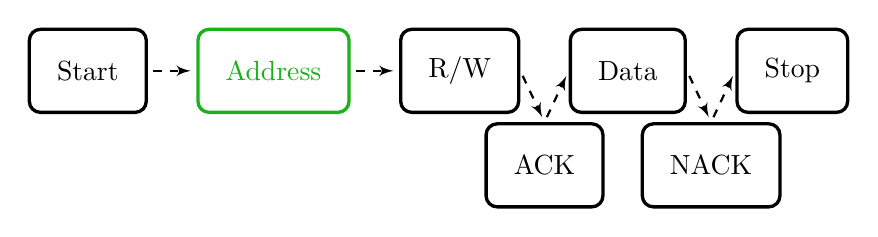
\begin{tikzpicture}[node distance=0.3cm, auto]
					\tikzset{%
						mynode/.style={rectangle,rounded corners,draw=black,top color=white, bottom color=white!50,very thick, inner sep=1em, minimum size=3em, text centered},
						invnode/.style={inner sep=0,minimum size=0}
					}
					\node[mynode](s){Start};
					\node[invnode, right=of s](i1){};
					\node[mynode,color=bettergreen, right=of i1](a){Address};
					\node[invnode, right=of a](i2){};
					\node[mynode, right=of i2](r){R/\textoverline{W}};
					\node[invnode, right=of r](i3){};
					\node[invnode, below of=i3](iv1){};
					\node[invnode, below of=iv1](iv2){};
					\node[invnode, below of=iv2](iv3){};
					\node[mynode, below of=iv3](ack1){ACK};
					\node[mynode, right=of i3](d){Data};
					\node[invnode, right=of d](i4){};
					\node[invnode, below of=i4](iv4){};
					\node[invnode, below of=iv4](iv5){};
					\node[invnode, below of=iv5](iv6){};
					\node[mynode, below of=iv6](ack2){NACK};
					\node[mynode, right=of i4](p){Stop};

					\draw[->, >=latex', shorten >=2pt, shorten <=2pt, thick, dashed] (s.east) to node[auto, swap] {}(a.west); 
					\draw[->, >=latex', shorten >=2pt, shorten <=2pt, thick, dashed] (a.east) to node[auto, swap] {}(r.west); 
					\draw[->, >=latex', shorten >=2pt, shorten <=2pt, thick, dashed] (r.east) to node[auto, swap] {}(ack1.north); 
					\draw[->, >=latex', shorten >=2pt, shorten <=2pt, thick, dashed] (ack1.north) to node[auto, swap] {}(d.west); 
					\draw[->, >=latex', shorten >=2pt, shorten <=2pt, thick, dashed] (d.east) to node[auto, swap] {}(ack2.north); 
					\draw[->, >=latex', shorten >=2pt, shorten <=2pt, thick, dashed] (ack2.north) to node[auto, swap] {}(p.west); 
				\end{tikzpicture}
			\end{figure}
		}
	%}}}
	%{{{
		\only<4>{%
			\begin{figure}
				\centering
				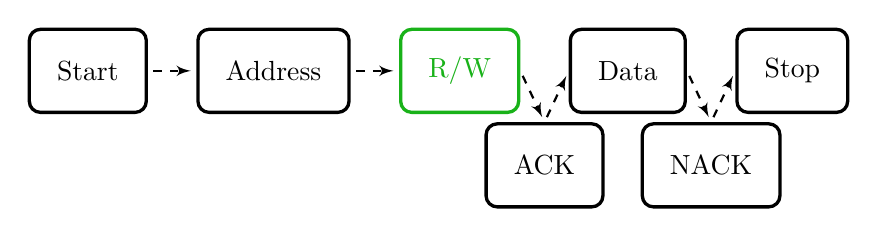
\begin{tikzpicture}[node distance=0.3cm, auto]
					\tikzset{%
						mynode/.style={rectangle,rounded corners,draw=black,top color=white, bottom color=white!50,very thick, inner sep=1em, minimum size=3em, text centered},
						invnode/.style={inner sep=0,minimum size=0}
					}
					\node[mynode](s){Start};
					\node[invnode, right=of s](i1){};
					\node[mynode, right=of i1](a){Address};
					\node[invnode, right=of a](i2){};
					\node[mynode,color=bettergreen, right=of i2](r){R/\textoverline{W}};
					\node[invnode, right=of r](i3){};
					\node[invnode, below of=i3](iv1){};
					\node[invnode, below of=iv1](iv2){};
					\node[invnode, below of=iv2](iv3){};
					\node[mynode, below of=iv3](ack1){ACK};
					\node[mynode, right=of i3](d){Data};
					\node[invnode, right=of d](i4){};
					\node[invnode, below of=i4](iv4){};
					\node[invnode, below of=iv4](iv5){};
					\node[invnode, below of=iv5](iv6){};
					\node[mynode, below of=iv6](ack2){NACK};
					\node[mynode, right=of i4](p){Stop};

					\draw[->, >=latex', shorten >=2pt, shorten <=2pt, thick, dashed] (s.east) to node[auto, swap] {}(a.west); 
					\draw[->, >=latex', shorten >=2pt, shorten <=2pt, thick, dashed] (a.east) to node[auto, swap] {}(r.west); 
					\draw[->, >=latex', shorten >=2pt, shorten <=2pt, thick, dashed] (r.east) to node[auto, swap] {}(ack1.north); 
					\draw[->, >=latex', shorten >=2pt, shorten <=2pt, thick, dashed] (ack1.north) to node[auto, swap] {}(d.west); 
					\draw[->, >=latex', shorten >=2pt, shorten <=2pt, thick, dashed] (d.east) to node[auto, swap] {}(ack2.north); 
					\draw[->, >=latex', shorten >=2pt, shorten <=2pt, thick, dashed] (ack2.north) to node[auto, swap] {}(p.west); 
				\end{tikzpicture}
			\end{figure}
		}
	%}}}
	%{{{
		\only<5>{%
			\begin{figure}
				\centering
				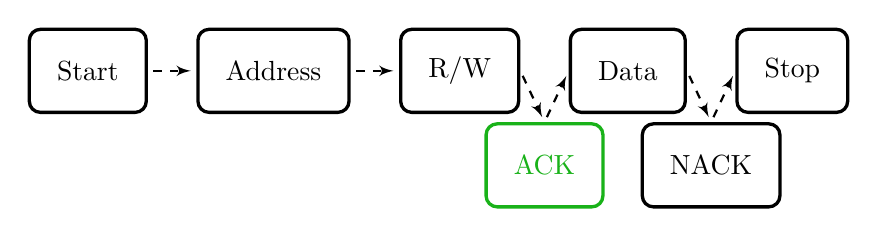
\begin{tikzpicture}[node distance=0.3cm, auto]
					\tikzset{%
						mynode/.style={rectangle,rounded corners,draw=black,top color=white, bottom color=white!50,very thick, inner sep=1em, minimum size=3em, text centered},
						invnode/.style={inner sep=0,minimum size=0}
					}
					\node[mynode](s){Start};
					\node[invnode, right=of s](i1){};
					\node[mynode, right=of i1](a){Address};
					\node[invnode, right=of a](i2){};
					\node[mynode, right=of i2](r){R/\textoverline{W}};
					\node[invnode, right=of r](i3){};
					\node[invnode, below of=i3](iv1){};
					\node[invnode, below of=iv1](iv2){};
					\node[invnode, below of=iv2](iv3){};
					\node[mynode,color=bettergreen, below of=iv3](ack1){ACK};
					\node[mynode, right=of i3](d){Data};
					\node[invnode, right=of d](i4){};
					\node[invnode, below of=i4](iv4){};
					\node[invnode, below of=iv4](iv5){};
					\node[invnode, below of=iv5](iv6){};
					\node[mynode, below of=iv6](ack2){NACK};
					\node[mynode, right=of i4](p){Stop};

					\draw[->, >=latex', shorten >=2pt, shorten <=2pt, thick, dashed] (s.east) to node[auto, swap] {}(a.west); 
					\draw[->, >=latex', shorten >=2pt, shorten <=2pt, thick, dashed] (a.east) to node[auto, swap] {}(r.west); 
					\draw[->, >=latex', shorten >=2pt, shorten <=2pt, thick, dashed] (r.east) to node[auto, swap] {}(ack1.north); 
					\draw[->, >=latex', shorten >=2pt, shorten <=2pt, thick, dashed] (ack1.north) to node[auto, swap] {}(d.west); 
					\draw[->, >=latex', shorten >=2pt, shorten <=2pt, thick, dashed] (d.east) to node[auto, swap] {}(ack2.north); 
					\draw[->, >=latex', shorten >=2pt, shorten <=2pt, thick, dashed] (ack2.north) to node[auto, swap] {}(p.west); 
				\end{tikzpicture}
			\end{figure}
		}
	%}}}
	%{{{
		\only<6>{%
			\begin{figure}
				\centering
				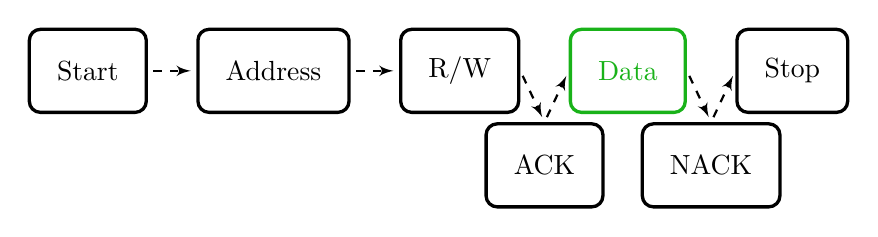
\begin{tikzpicture}[node distance=0.3cm, auto]
					\tikzset{%
						mynode/.style={rectangle,rounded corners,draw=black,top color=white, bottom color=white!50,very thick, inner sep=1em, minimum size=3em, text centered},
						invnode/.style={inner sep=0,minimum size=0}
					}
					\node[mynode](s){Start};
					\node[invnode, right=of s](i1){};
					\node[mynode, right=of i1](a){Address};
					\node[invnode, right=of a](i2){};
					\node[mynode, right=of i2](r){R/\textoverline{W}};
					\node[invnode, right=of r](i3){};
					\node[invnode, below of=i3](iv1){};
					\node[invnode, below of=iv1](iv2){};
					\node[invnode, below of=iv2](iv3){};
					\node[mynode, below of=iv3](ack1){ACK};
					\node[mynode,color=bettergreen, right=of i3](d){Data};
					\node[invnode, right=of d](i4){};
					\node[invnode, below of=i4](iv4){};
					\node[invnode, below of=iv4](iv5){};
					\node[invnode, below of=iv5](iv6){};
					\node[mynode, below of=iv6](ack2){NACK};
					\node[mynode, right=of i4](p){Stop};

					\draw[->, >=latex', shorten >=2pt, shorten <=2pt, thick, dashed] (s.east) to node[auto, swap] {}(a.west); 
					\draw[->, >=latex', shorten >=2pt, shorten <=2pt, thick, dashed] (a.east) to node[auto, swap] {}(r.west); 
					\draw[->, >=latex', shorten >=2pt, shorten <=2pt, thick, dashed] (r.east) to node[auto, swap] {}(ack1.north); 
					\draw[->, >=latex', shorten >=2pt, shorten <=2pt, thick, dashed] (ack1.north) to node[auto, swap] {}(d.west); 
					\draw[->, >=latex', shorten >=2pt, shorten <=2pt, thick, dashed] (d.east) to node[auto, swap] {}(ack2.north); 
					\draw[->, >=latex', shorten >=2pt, shorten <=2pt, thick, dashed] (ack2.north) to node[auto, swap] {}(p.west); 
				\end{tikzpicture}
			\end{figure}
		}
	%}}}
	%{{{
		\only<7>{%
			\begin{figure}
				\centering
				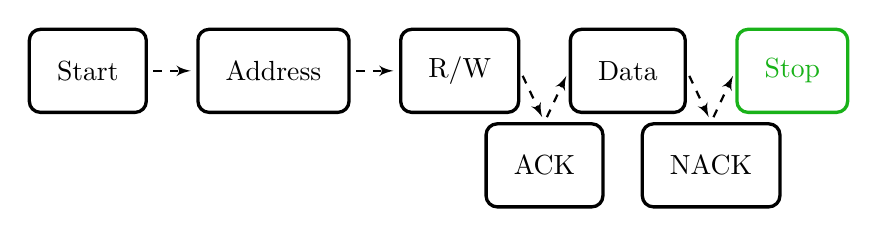
\begin{tikzpicture}[node distance=0.3cm, auto]
					\tikzset{%
						mynode/.style={rectangle,rounded corners,draw=black,top color=white, bottom color=white!50,very thick, inner sep=1em, minimum size=3em, text centered},
						invnode/.style={inner sep=0,minimum size=0}
					}
					\node[mynode](s){Start};
					\node[invnode, right=of s](i1){};
					\node[mynode, right=of i1](a){Address};
					\node[invnode, right=of a](i2){};
					\node[mynode, right=of i2](r){R/\textoverline{W}};
					\node[invnode, right=of r](i3){};
					\node[invnode, below of=i3](iv1){};
					\node[invnode, below of=iv1](iv2){};
					\node[invnode, below of=iv2](iv3){};
					\node[mynode, below of=iv3](ack1){ACK};
					\node[mynode, right=of i3](d){Data};
					\node[invnode, right=of d](i4){};
					\node[invnode, below of=i4](iv4){};
					\node[invnode, below of=iv4](iv5){};
					\node[invnode, below of=iv5](iv6){};
					\node[mynode, below of=iv6](ack2){NACK};
					\node[mynode,color=bettergreen, right=of i4](p){Stop};

					\draw[->, >=latex', shorten >=2pt, shorten <=2pt, thick, dashed] (s.east) to node[auto, swap] {}(a.west); 
					\draw[->, >=latex', shorten >=2pt, shorten <=2pt, thick, dashed] (a.east) to node[auto, swap] {}(r.west); 
					\draw[->, >=latex', shorten >=2pt, shorten <=2pt, thick, dashed] (r.east) to node[auto, swap] {}(ack1.north); 
					\draw[->, >=latex', shorten >=2pt, shorten <=2pt, thick, dashed] (ack1.north) to node[auto, swap] {}(d.west); 
					\draw[->, >=latex', shorten >=2pt, shorten <=2pt, thick, dashed] (d.east) to node[auto, swap] {}(ack2.north); 
					\draw[->, >=latex', shorten >=2pt, shorten <=2pt, thick, dashed] (ack2.north) to node[auto, swap] {}(p.west); 
				\end{tikzpicture}
			\end{figure}
		}
	%}}}
	\end{minipage}
	\begin{columns}
		\column{0.4\textwidth}
		\begin{minipage}[c][.4\textheight][c]{\linewidth}
			\begin{figure}
			%\includegraphics[width=\textwidth,height=0.8\textheight,keepaspectratio]{#2}
				%\only<1>{
\includegraphics[height=0.45\textheight]{dummy}}%
				\only<2>{
\includegraphics[height=0.45\textheight]{dummy}}%
				%\only<3>{
\includegraphics[height=0.45\textheight]{dummy}}%
				%\only<4>{
\includegraphics[height=0.45\textheight]{dummy}}%
				\only<5>{
\includegraphics[height=0.45\textheight]{dummy}}%
				%\only<6>{
\includegraphics[height=0.45\textheight]{dummy}}%
				\only<7>{
\includegraphics[height=0.45\textheight]{dummy}}%
			\end{figure}
		\end{minipage}
		\column{0.6\textwidth}
		\begin{minipage}[c][.4\textheight][c]{\linewidth}
			\begin{tabular}{p{0.15cm} p{5cm}}
				\only<1>{\\}
				\only<1>{\\}
				\only<1>{\\}
				\only<2>{\greenbullet & \scl high\\}
				\only<2>{\greenbullet & Master injects negative Edge on \sda\\}
				\only<2>{\\}
				\only<3>{\greenbullet & Seven bits of address are transmitted\\}
				\only<3>{\greenbullet & Some addresses are reserved\\}
				\only<3>{\\}
				\only<4>{\greenbullet & ``1'' for reading\\}
				\only<4>{\greenbullet & ``0'' for writing\\}
				\only<4>{\\}
				\only<5>{\greenbullet & Transmitter releases the \sda line\\}
				\only<5>{\greenbullet & Receiver pulls \sda low to acknowledge\\}
				\only<5>{\\}
				\only<6>{\greenbullet & Transmitter sends one byte of data                  \\}
				\only<6>{\greenbullet & It may send the next byte if receiver acknowledges  \\}
				\only<6>{\greenbullet & When receiver not-acknowledges the transmission ends\\}
				\only<7>{\greenbullet & \scl high\\}
				\only<7>{\greenbullet & Master injects Positive-going Edge on \sda\\}
				\only<7>{\\}
			\end{tabular}
		\end{minipage}
	\end{columns}
\end{frame}
%}}}

%{{{
\begin{frame}[fragile]{\twi Protocol Example/1}
%	\begin{changemargin}{-1cm}{+1cm}
%%%%\begin{tikztimingtable}[%
%%%%		timing/dslope=0.2,
%%%%		timing/dslope=0.2,
%%%%		%timing/name/.style={font=\sffamily\scriptsize},
%%%%		%timing/d/text/.style={font=\sffamily\tiny},
%%%%		%rayz/.style={timing/z/.append style={gray}},
%%%%		%iming/n/.style={rectangle},
%%%%		timing/metachar={{K}[2]{#1h!{++(0,-.5\yunit)} N[rectangle,scale=.3]{#2}!{++(0,+.5\yunit)} #1h}},
%%%%		timing/metachar={{J}[2]{#1l!{++(0,+.5\yunit)} N[rectangle,scale=.3]{#2}!{++(0,-.5\yunit)} #1l}},
%%%%	]
%%%%	SDA$_{Master}$ & hL DD{A}{} d[dotted]D;d{}DD{A}{} HK{R}{} HH HH HH; h[dotted]H;h HH HH HK{NACK} LLhH \\
%%%%	SDA$_{Slave}$  & hH HH     ;h[dotted]H;h  HH      HH        LJ{ACK} HH DD{D}{} d[dotted]D;d{}DD{D}{} DD{D}{} HK{} HHhH \\
%%%%	SDA            & hL DD{A}{} d[dotted]D;d{}DD{A}{} HK{R}{} LJ{ACK} HH DD{D}{} d[dotted]D;d{}DD{D}{} DD{D}{} HK{NACK} LLhH \\
%%%%	SCL & HLK{1} L;  [dotted]L;L   K{7} L  K{8} L    K{9}   LL LK{1} L; [dotted]L;L   K{7} L  K{8} L  K{9}   LLHH \\
%%%%	\extracode
%%%%	\begin{background}
%%%%		\vertlines[help lines]{}
%%%%		\horlines[help lines]{}
%%%%		\show\horlines
%%%%	%	\draw [->,>=latex] (0,-\nrows-1) -- (\twidth+1,-\nrows-1);
%%%%	%	\foreach \n in {0,1,...,\twidth}
%%%%	%	\draw (\n,-\nrows-1+.1) -- +(0,-.2)
%%%%	%	node [below,inner sep=2pt] {\scalebox{.75}{\tiny\n}};
%%%%	\end{background}
%%%%	%\tablegrid[black!25]
%%%%\end{tikztimingtable}
%%%%%	\end{changemargin}
			\begin{figure}
				
\includegraphics[width=\textwidth,height=0.8\textheight,keepaspectratio]{dummy}
				\caption{Simple \twi read on default register}
			\end{figure}
\end{frame}
%}}}

%{{{
\begin{frame}[fragile]{\twi Protocol Example/2}
	\begin{changemargin}{-0.7cm}{+1cm}
%%%%		\resizebox{\linewidth+1.5cm}{!}{%
%%%%			\begin{tikztimingtable}[%
%%%%					timing/dslope=0.2,
%%%%					timing/dslope=0.2,
%%%%		%timing/name/.style={font=\sffamily\scriptsize},
%%%%		%timing/d/text/.style={font=\sffamily\tiny},
%%%%		%rayz/.style={timing/z/.append style={gray}},
%%%%		%iming/n/.style={rectangle},
%%%%					timing/metachar={{K}[2]{#1h!{++(0,-.5\yunit)} N[rectangle,scale=.3]{#2}!{++(0,+.5\yunit)} #1h}},
%%%%					timing/metachar={{J}[2]{#1l!{++(0,+.5\yunit)} N[rectangle,scale=.3]{#2}!{++(0,-.5\yunit)} #1l}},
%%%%				]
%%%%				SDA$_{Master}$ & hL DD{A}{} d[dotted]D;d{}DD{A}{} HK{R}{} HH HH HH; h[dotted]H;h HH HH HK{NACK} HHL                       DD{A}{} d[dotted]D;d{}DD{A}{} LJ{W}{} HK{}    HH DD{D}{} d[dotted]D;d{}DD{D}{} DD{D}{} HK{}     LLhH\\
%%%%				SDA$_{Slave1}$  & hH HH     ;h[dotted]H;h  HH      HH        LJ{ACK} HH DD{D}{} d[dotted]D;d{}DD{D}{} DD{D}{} HK{} HHhH HHHHHHHHHHHHHHHHHHHHHHHHH\\
%%%%				SDA$_{Slave2}$  & hH HH     ;h[dotted]H;h  HH      HH   HH HH HH h     ;h[dotted]H;h  HH  HH HHHH H HH     ;h[dotted]H;  HH      HH        LJ{ACK} HH HH; h[dotted]H;h HH HH HK{NACK} HHhH \\
%%%%				SDA            & hL DD{A}{} d[dotted]D;d{}DD{A}{} HK{R}{} LJ{ACK} HH DD{D}{} d[dotted]D;d{}DD{D}{} DD{D}{} HK{NACK} HHL DD{A}{} d[dotted]D;d{}DD{A}{} LJ{W}{} LJ{ACK} HH DD{D}{} d[dotted]D;d{}DD{D}{} DD{D}{} HK{NACK} LLhH\\
%%%%				SCL & HLK{1} L;  [dotted]L;L   K{7} L  K{8} L    K{9}   LL LK{1} L; [dotted]L;L   K{7} L  K{8} L  K{9}   LL   HLK{1} L;  [dotted]L;L   K{7} L  K{8} L    K{9}   LL LK{1} L; [dotted]L;L   K{7} L  K{8} L  K{9}   LLHH \\
%%%%				\extracode
%%%%				\begin{background}
%%%%					\vertlines[help lines]{}
%%%%					\horlines[help lines]{}
%%%%					\show\horlines
%%%%	%	\draw [->,>=latex] (0,-\nrows-1) -- (\twidth+1,-\nrows-1);
%%%%	%	\foreach \n in {0,1,...,\twidth}
%%%%	%	\draw (\n,-\nrows-1+.1) -- +(0,-.2)
%%%%	%	node [below,inner sep=2pt] {\scalebox{.75}{\tiny\n}};
%%%%				\end{background}
%%%%	%\tablegrid[black!25]
%%%%			\end{tikztimingtable}
%%%%		}
			\begin{figure}
				
\includegraphics[width=\textwidth,height=0.8\textheight,keepaspectratio]{dummy}
				\caption{Example of repeated start}
			\end{figure}
			%Example of repeated Start

			\vspace{5mm}


%%%%		\resizebox{\linewidth+1.5cm}{!}{%
%%%%			\begin{tikztimingtable}[%
%%%%					timing/dslope=0.2,
%%%%					timing/dslope=0.2,
%%%%		%timing/name/.style={font=\sffamily\scriptsize},
%%%%		%timing/d/text/.style={font=\sffamily\tiny},
%%%%		%rayz/.style={timing/z/.append style={gray}},
%%%%		%iming/n/.style={rectangle},
%%%%					timing/metachar={{K}[2]{#1h!{++(0,-.5\yunit)} N[rectangle,scale=.3]{#2}!{++(0,+.5\yunit)} #1h}},
%%%%					timing/metachar={{J}[2]{#1l!{++(0,+.5\yunit)} N[rectangle,scale=.3]{#2}!{++(0,-.5\yunit)} #1l}},
%%%%				]
%%%%				SDA$_{Slave}$  & hH HH     ;h[dotted]H;h  HH      HH        LJ{ACK} HH DD{D}{} d[dotted]D;d{}DD{D}{} DD{D}{} HK{}   HH DD{D}{} d[dotted]D;d{}DD{D}{} DD{D}{} HK{}     HH DD{D}{} d[dotted]D;d{}DD{D}{} DD{D}{} HK{}                HHhH \\
%%%%				SDA            & hL DD{A}{} d[dotted]D;d{}DD{A}{} HK{R}{} LJ{ACK} HH DD{D}{} d[dotted]D;d{}DD{D}{} DD{D}{} LJ{ACK}         HH DD{D}{} d[dotted]D;d{}DD{D}{} DD{D}{} LJ{ACK}                   HH DD{D}{} d[dotted]D;d{}DD{D}{} DD{D}{} HK{NACK}              LLhH \\
%%%%				SDA$_{Master}$ & hL DD{A}{} d[dotted]D;d{}DD{A}{} HK{R}{} HH HH HH; h[dotted]H;h HH HH LJ{ACK}      HH HH; h[dotted]H;h HH  HH    LJ{ACK}   HH HH ; h[dotted]H;h HH HH HK{NACK}     LLhH \\
%%%%				SCL & HLK{1} L;  [dotted]L;L   K{7} L  K{8} L    K{9}   LL LK{1} L; [dotted]L;L   K{7} L  K{8} L  K{9} LL LK{1} L;  [dotted]L;L   K{7} L  K{8} L    K{9}   LL LK{1} L; [dotted]L;L   K{7} L  K{8} L  K{9}  LLHH \\
%%%%				\extracode
%%%%				\begin{background}
%%%%					\vertlines[help lines]{}
%%%%					\horlines[help lines]{}
%%%%					\show\horlines
%%%%	%	\draw [->,>=latex] (0,-\nrows-1) -- (\twidth+1,-\nrows-1);
%%%%	%	\foreach \n in {0,1,...,\twidth}
%%%%	%	\draw (\n,-\nrows-1+.1) -- +(0,-.2)
%%%%	%	node [below,inner sep=2pt] {\scalebox{.75}{\tiny\n}};
%%%%				\end{background}
%%%%	%\tablegrid[black!25]
%%%%			\end{tikztimingtable}
%%%%		}
			\begin{figure}
				
\includegraphics[width=\textwidth,height=0.8\textheight,keepaspectratio]{dummy}
				\caption{Example of multi-byte transmission}
			\end{figure}
			%Example of multi-byte transmission
	\end{changemargin}
\end{frame}
%}}}

%{{{
\begin{frame}[fragile]{\twi Clock Stretching}
		\begin{minipage}[c][.4\textheight][c]{\linewidth}
			\begin{tabular}{p{0.15cm} l}
				\greenbullet & No fixed speed: Any device may slow down the transmission\\
				\greenbullet & Master pauses switching of \scl \textrightarrow transmission is paused\\
				\greenbullet & Slave holds \scl low \textrightarrow master waits for release\\
			\end{tabular}
		\end{minipage}
	\begin{changemargin}{-0.5cm}{+1cm}
%%%%		\begin{tikztimingtable}[%
%%%%				timing/dslope=0.2,
%%%%				timing/dslope=0.2,
%%%%		%timing/name/.style={font=\sffamily\scriptsize},
%%%%		%timing/d/text/.style={font=\sffamily\tiny},
%%%%		%rayz/.style={timing/z/.append style={gray}},
%%%%		%iming/n/.style={rectangle},
%%%%				timing/metachar={{K}[2]{#1h!{++(0,-.5\yunit)} N[rectangle,scale=.3]{#2}!{++(0,+.5\yunit)} #1h}},
%%%%				timing/metachar={{J}[2]{#1l!{++(0,+.5\yunit)} N[rectangle,scale=.3]{#2}!{++(0,-.5\yunit)} #1l}},
%%%%			]
%%%%			SDA            & hL DD{A}{} d[dotted]D;d{}DD{A}{} DD{A}{} HK{R}{} LJ{ACK} HH DD{D}{} d[dotted]D;d{}DD{D}{} DD{D}{} HK{NACK} LLhH \\
%%%%			SCL & HLK{1} L;  [dotted]L;L  K{6} L  K{7} L  K{8} L    K{9}   LL LK{1} L; [dotted]L;L   K{7} L  K{8} L  K{9}   LLHH \\
%%%%			\\
%%%%			%SDA$_{Master}$ & hL DD{A}{} d[dotted]D;d{} DD{A}{} DDDDDDDD{A}{} HK{R}{} HH HH HH; h[dotted]H;h HH HH HK{NACK} LLhH \\
%%%%			%SDA$_{Slave}$  & hH HH     ;h[dotted]H;h  HH  HH  HH HH HH  HH        LJ{ACK} HH DD{D}{} d[dotted]D;d{}DD{D}{} DD{D}{} HK{} HHhH \\
%%%%			SDA            & hL DD{A}{} d[dotted]D;d{}DD{A}{} DDDDDDDD{A}{} HK{R}{} LJ{ACK} HH DD{D}{} d[dotted]D;d{}DD{D}{} DD{D}{} HK{NACK} LLhH \\
%%%%			SCL$_{Master}$ & HLK{1} L;  [dotted]L;L K{6} L HHHHHH K{7} L  K{8} L    K{9}   LL LK{1} L; [dotted]L;L   K{7} L  K{8} L  K{9}   LLHH \\
%%%%			SCL$_{Slave}$  & HHH H;  [dotted]H;H    H    J{s}J{t}J{r}J{e}J{c}J{h} L H H  H H    H   HH HH H; [dotted]H;H   H H  H H  H   HHHH \\
%%%%			SCL           & HLK{1} L;  [dotted]L;L  K{6} LLLLLL L K{7} L  K{8} L    K{9}   LL LK{1} L; [dotted]L;L   K{7} L  K{8} L  K{9}   LLHH \\
%%%%			\extracode
%%%%			\begin{background}
%%%%				\vertlines[help lines]{}
%%%%				\horlines[help lines]{}
%%%%				\show\horlines
%%%%	%	\draw [->,>=latex] (0,-\nrows-1) -- (\twidth+1,-\nrows-1);
%%%%	%	\foreach \n in {0,1,...,\twidth}
%%%%	%	\draw (\n,-\nrows-1+.1) -- +(0,-.2)
%%%%	%	node [below,inner sep=2pt] {\scalebox{.75}{\tiny\n}};
%%%%			\end{background}
%%%%	%\tablegrid[black!25]
%%%%		\end{tikztimingtable}
			\begin{figure}
				
\includegraphics[width=\textwidth,height=0.8\textheight,keepaspectratio]{dummy}
				\caption{Upper diagram: no stretching, lower diagram: with stretching}
			\end{figure}
	\end{changemargin}
\end{frame}
%}}}

%{{{
\begin{frame}[fragile]{\twi Collision Detection \& Bus Arbitration}
	\begin{minipage}[c][.4\textheight][c]{\linewidth}
		\begin{tabular}{p{0.15cm} l}
			\greenbullet & Two devices issue start condition \textrightarrow become master of the bus\\
			\greenbullet & Both transmit address and possibly data\\
			\greenbullet & One master sends ``1'', one sends ``0''\\
			\greenbullet & The master sending ``1'' notices the discrepancy between its output and the bus \textrightarrow loses arbitration\\
			\greenbullet & A master that lost bus arbitration switches to slave mode\\
			\\
		\end{tabular}
%%%%		\begin{tikztimingtable}[%
%%%%				timing/dslope=0.2,
%%%%				timing/dslope=0.2,
%%%%		%timing/name/.style={font=\sffamily\scriptsize},
%%%%		%timing/d/text/.style={font=\sffamily\tiny},
%%%%		%rayz/.style={timing/z/.append style={gray}},
%%%%		%iming/n/.style={rectangle},
%%%%				timing/metachar={{K}[2]{#1h!{++(0,-.5\yunit)} N[rectangle,scale=.3]{#2}!{++(0,+.5\yunit)} #1h}},
%%%%				timing/metachar={{J}[2]{#1l!{++(0,+.5\yunit)} N[rectangle,scale=.3]{#2}!{++(0,-.5\yunit)} #1l}},
%%%%			]
%%%%			SDA$_{Master1}$ & hL HH      LL     LL      HH     HH      LL     LL      HK{R}{} HH HH HH; h[dotted]H;h  HK{NACK} LLhH \\
%%%%			SDA$_{Master2}$ & hL HH      LL     LL      HH     HH      HH     HH      HH      LJ{ACK} HH DD{D}{} d[dotted]D;d{} HK{} HHhH \\
%%%%			SDA             & hL HH      LL     LL      HH     HH      LL     LL      HK{R}{} LJ{ACK} HH DD{D}{} d[dotted]D;d{} HK{NACK} LLhH \\
%%%%			SCL             & HL K{1} L  K{2} L K{3} L  K{4} L K{5} L  K{6} L K{7} L  K{8} L  K{9}   LL LK{1} L; [dotted]L;L     K{9}   LLHH \\
%%%%			\\
%%%%			\extracode
%%%%			\begin{background}
%%%%				\vertlines[help lines]{}
%%%%				\horlines[help lines]{}
%%%%				\show\horlines
%%%%	%	\draw [->,>=latex] (0,-\nrows-1) -- (\twidth+1,-\nrows-1);
%%%%	%	\foreach \n in {0,1,...,\twidth}
%%%%	%	\draw (\n,-\nrows-1+.1) -- +(0,-.2)
%%%%	%	node [below,inner sep=2pt] {\scalebox{.75}{\tiny\n}};
%%%%			\end{background}
%%%%	%\tablegrid[black!25]
%%%%		\end{tikztimingtable}
			\begin{figure}
				
\includegraphics[width=\textwidth,height=0.8\textheight,keepaspectratio]{dummy}
			\end{figure}
		\begin{tabular}{p{0.15cm} l}
			\greenbullet & Second master became slave before any race condition occured\\
			\greenbullet & \textrightarrow no data loss\\
		\end{tabular}
	\end{minipage}
\end{frame}
%}}}

%{{{
\begin{frame}{\twi 10-bit Addressing}
	\begin{minipage}[c][.4\textheight][c]{\linewidth}
		\begin{tabular}{p{0.15cm} l}
			\greenbullet & 7-bit addressing means 128 addresses\\
			\greenbullet & 16 addresses reserved \textrightarrow only 112 addresses free\\
			\greenbullet & More addresses needed \textrightarrow 10-bit-addressing:\\
			             & First byte: 11110 + first 2 bits of 10-bit address + R/W-bit\\
						 & Second byte: Remaining 8 bits of slave address\\
						 & Rest of transmission as usual\\
			\\
		\end{tabular}
			\begin{figure}
				
\includegraphics[width=\textwidth,height=0.8\textheight,keepaspectratio]{dummy}
				\source{Adapted from \url{``UM10204 I2C-bus specification and user manual Rev. 6'', 2014}}
			\end{figure}
	\end{minipage}
\end{frame}
%}}}

%{{{
\begin{frame}{\twi Higher Speeds}
	\begin{changemargin}{-0.7cm}{+1cm}
		\begin{tabular}{p{0.15cm} p{2.7cm} l}
			\greenbullet & Standard Mode   & Up to 100kbit/s\\
			\greenbullet & Fast Mode       & Up to 400kbit/s\\
		                 &                 & Fully compatible with Standard Mode\\
			\greenbullet & Fast Mode Plus  & Up to 1Mbit/s\\
			             &                 & Timing loosened, more drive strength\\
			\greenbullet & High Speed Mode & Up to 3.4Mbit/s\\
			&                 & A number of changes:\\
			&                 & \greencirc Pull-up current sources in each device\\
			&                 & \greencirc Schmitt-trigger inputs for spike suppression\\
			&                 & \greencirc Clock stretching only after \ack bit\\
			&                 & \greencirc \textrightarrow special initiation: master-code\\
			&                 & ``00001XX'' ``X'' transmitted in Fast Mode\\
			&                 & Bus arbitration only during master-code transfer\\
			\\
		\end{tabular}
	\end{changemargin}
\end{frame}
%}}}

%{{{
\begin{frame}{\twi High Speed Mode Electrical Setup}
	\begin{changemargin}{-0.7cm}{+1cm}
		\begin{figure}
			
\includegraphics[width=\textwidth,height=0.9\textheight,keepaspectratio]{dummy}
			\source{Adapted from \href{http://www.cs.unc.edu/Research/stc/FAQs/Interfaces/I2C-BusSpec-V2.1.pdf}{``The I\textsuperscript{2}C-Bus Specification v. 2.1'', 2000}}
		\end{figure}
	\end{changemargin}
\end{frame}
%}}}

%{{{
\begin{frame}{\twi Ultra Fast Mode}
	\begin{changemargin}{-0.7cm}{+1cm}
		\begin{tabular}{p{0.15cm} p{2.7cm} l}
			\greenbullet & Ultra Fast Mode & Up to 5Mbit/s\\
			             &                 & Not compatible\\
			&                 & Changes:\\
			&                 & \greencirc Unidirectional Protocol\\
			&                 & \greencirc Push-Pull output stages\\
			&                 & \greencirc Rest of protocol remains mostly the same\\
			\\
		\end{tabular}
	\end{changemargin}
\end{frame}
%}}}




\section[Measurements]{Practical Part}

%{{{
\begin{frame}{Practical Part}
	\begin{columns}
		\column{0.4\textwidth}
		\begin{itemize}
			\item Goal: Measure an \twi transaction
			\item A Raspberry Pi is connected to a lab card
			\item Measurement done with a temperature sensor on the card
		\end{itemize}
		\column{0.6\textwidth}
		\begin{figure}
			
\includegraphics[width=0.9\textwidth,height=0.7\textheight,keepaspectratio]{dummy}
			\source{\url{http://static.trustedreviews.com/94/00002d03f/1a88_orh350w620/Raspberry-Pi-B-Plus-model.jpg}}
		\end{figure}
		\vspace{2mm}
	\end{columns}
\end{frame}
%}}}

%{{{
\begin{frame}{Hardware Setup}
	\begin{columns}
		\column{0.6\textwidth}
		\begin{figure}
			
\includegraphics[width=0.9\linewidth]{dummy}
		\end{figure}
		\column{0.4\textwidth}
		\begin{itemize}
			\item Raspberry Pi drives \twi bus multiplexer LTC4306
			\item LTC4306 connected to temperature sensor MAX6657
			\item Oscilloscope attached to \twi bus on sensor
		\end{itemize}
	\end{columns}
\end{frame}
%}}}

%{{{
\begin{frame}{Software Setup}
	\begin{minipage}[c][.4\textheight][c]{\linewidth}
		\begin{tabular}{p{0.15cm} p{3.5cm} l}
			\greenbullet & Load Kernel Modules & \texttt{i2c-bcm2708} \& \texttt{i2c-dev}\\
			\greenbullet & Load package & \texttt{i2c-tools}\\
			\greenbullet & Start terminal session:\\
			\\
		\end{tabular}
	\end{minipage}
\end{frame}
%}}}

%{{{
\begin{frame}[fragile]{Software Session}
	\begin{minipage}[c][.4\textheight][c]{\linewidth}
		\begin{minted}[fontsize=\small]{bash}
			# Tell the multiplexer to connect the
			# correct bus to the pi.
			pi@raspberrypi ~ $ i2cset 1 73 3 64
			WARNING! This program can confuse your
			I2C bus, cause data loss and worse!
			I will write to device file
			/dev/i2c-1, chip address 0x49, data
			address 0x03, data 0x40, mode byte.
			Continue? [Y/n] y
			# Read the temperature sensor.
			pi@raspberrypi ~ $ i2cget -y 1 76 0
			0x1b
			# A thumb was placed on the sensor
			# to warm it up a little
			pi2@raspberrypi ~ $ i2cget -y 1 76 0
			0x1d
		\end{minted}
	\end{minipage}
\end{frame}
%}}}

%{{{
\begin{frame}{\twi Measurement}
	\begin{changemargin}{-0.6cm}{+1cm}
		\begin{figure}
			
\includegraphics[width=1.1\textwidth]{dummy}
		\end{figure}
	\end{changemargin}
\end{frame}
%}}}

\section[Conclusion]{Conclusion}


%{{{
\begin{frame}[fragile]{Comparison of SPI an \twi}
	\begin{figure}[!t]
		\centering
		\resizebox{3in}{!}}}


%{{{
\begin{frame}{Conclusion}
		\begin{itemize}
			\item Both SPI and \twi very mature busses
			\item Nevertheless up to date
			\item Low pin count, low speeds
			\item SPI used for data connections mostly
			\item \twi prevalently used for configuration centric communication
		\end{itemize}
\end{frame}
%}}}

%{{{ References

\center{References}
\tiny
\begin{thebibliography}{9}
	\bibitem{spi_mc68hc11a8}
		Datasheet of the Motorola MC68HC11A8 microcontroller describing the SPI bus.\\
		Last downloaded 2014-01-10\\
		\url{http://cache.freescale.com/files/microcontrollers/doc/data_sheet/MC68HC11A8.pdf}

	\bibitem{spi_c68hcp11a1vp}
		Datasheet of the Motorola MC68HCP11A1VP microcontroller\\
		Last downloaded 2014-01-10\\
		\url{http://pdf.datasheetcatalog.com/datasheet/motorola/MC68HCP11A1VP.pdf}

	\bibitem{spi_blockguide}
		SPI Block Guide V03.06\\
		Last downloaded 2014-01-10\\
		\url{http://www.ee.nmt.edu/~teare/ee308l/datasheets/S12SPIV3.pdf}

	\bibitem{microwire}
		Datasheet detailing Microwire\\
		Last downloaded 2014-01-11\\
		\url{http://www.ti.com/lit/an/snoa743/snoa743.pdf}

	\bibitem{i2c_standard_v2.1}
		Phillips Semiconductors: The \twi-Bus Specification, 2000\\
		Last downloaded 2014-01-10\\
		\url{http://www.cs.unc.edu/Research/stc/FAQs/Interfaces/I2C-BusSpec-V2.1.pdf}

	\bibitem{i2c_standard}
		NXP Semiconductors: UM10204 I2C-bus specification and user manual\\
		Last downloaded 2014-01-10\\
		\url{http://www.nxp.com/documents/user_manual/UM10204.pdf}

	\bibitem{pmbus}
		Homepage for PMBus, detailing it's connection to \twi\\
		Last visited 2014-01-11\\
		\url{http://pmbus.org/about/pmbusancestry}

	\bibitem{smbus}
		Specification of SMBus\\
		Last downloaded 2014-01-11\\
		\url{http://smbus.org/specs/smbus20.pdf}

	\bibitem{twi1}
		Homepage about \twi detailing TWI\\
		Last visited 2014-01-11\\
		\url{http://www.i2c-bus.org/twi-bus}

	\bibitem{twi2}
		Example of a datasheet using the term ``Two Wire Interface" instead of \twi\\
		Last downloaded 2014-01-11\\
		\url{http://www.atmel.com/Images/2466S.pdf}


\end{thebibliography}
%}}}

%{{{ END

\begin{frame}
	{\Huge End}
	Any Questions?
\end{frame}
%}}}


\end{document}
%}}}
